\chapter{АЛГОРИТМ МОДУЛЯ СКАНИРОВАНИЯ}\label{chap:algorithms}
    \section{Этапы работы алгоритма}
        Задача алгоритма заключается в преобразовании входных данных -- видео процесса сканирования и dxf файла с заданным контуром -- в gcode файл. Gcode файл это последовательность инструкций для принтера написанных особым образом. Файл формата dxf это векторное изображение некоторого произвольного рисунка, которое необходимо нанести на изделия в сцене.
        В целом алгоритм модуля состоит из четырёх операций:
        \begin{enumerate}
            \item Обработка видео/Получение облака точек
            \item Поиск объектов в облаке
            \item Подготовка dxf файла
            \item Генерация gcode файла
        \end{enumerate}
        
        Последовательность операций отражена в блок-схеме на рисунке \ref{pic:general_scheme}.
        \begin{figure}[h]
            \centering
            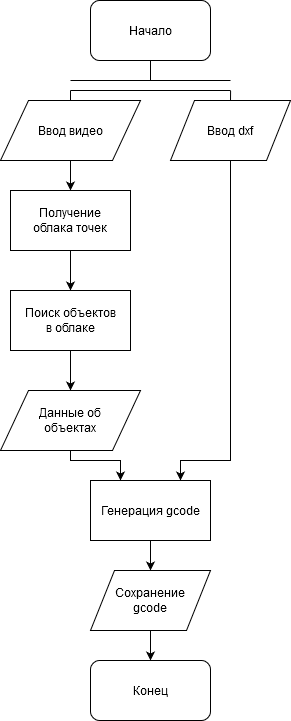
\includegraphics[width=0.5\linewidth]{general scheme}
            \caption{Обобщённая блок схема алгоритма модуля}
            \label{pic:general_scheme}
        \end{figure}
         При запуске алгоритма на вход передаются видео со сканера и dxf файл, а также загружаются дополнительные данные индивидуальные для принтера (конфиги, на схеме не показано). После этого запускаются этапы обработки видео и dxf файла. Эти этапы независимы и могут выполняться параллельно. Этап обработки видео включает в себя предобработку каждого кадра, затем выделение лазера в кадре, расчёт координат по формулам из главы \ref{chap:math}. Результатом этого этапа является облако точек сцены. Оно передаётся в следующий блок для поиска объектов. Цель этого этапа в получении положений и ориентаций объектов в сцене. Затем данные об объектах и подготовленный рисунок передаются в последний блок алгоритма, где из них генерируется файл инструкций для принтера которые задают последовательность печати рисунка из dxf файла на каждый найденный объект в сцене.
    \section{Блок обработки видео}
        Как уже было сказано, блок обработки видео включает в себя следующие шаги, которые выполняются для каждого кадра видео:
        \begin{enumerate}
            \item Предобработка кадра
            \item Выделение лазера
            \item Расчёт координат
        \end{enumerate}
        
        \begin{wrapfigure}{r}{0.5\linewidth}
            \centering
            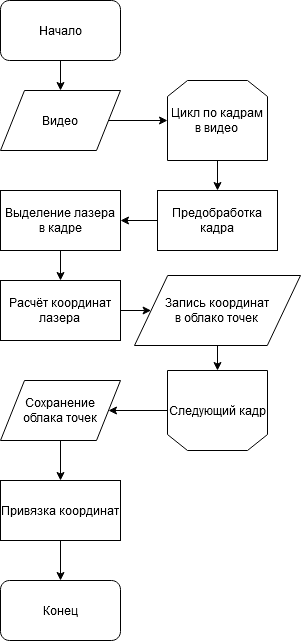
\includegraphics[height=0.45\textheight, keepaspectratio]{video_processing}
            \caption{Обобщённая блок схема обработки видео}
            \label{pic:video_processing}
        \end{wrapfigure}
        После этого облако точек сохраняется в памяти и производится привязка координат к системе принтера. Этот этап необходим, потому что в виду аппаратных ограничений сканирование в общем случае начинается в произвольном месте до рабочей поверхности и получить точную координату не представляется возможным. Поэтому данная задача решается программными средствами.
        \sloppy Результатом работы алгоритма становится облако точек, представляющее из себя матрицу размерностью $ (\mbox{\textit{количество кадров}}\times\mbox{\textit{ширина кадра}}) $ где в каждой ячейке записана координата соответствующая этой точке. Таким образом облако точек одновременно является картой глубины сцены.
        
        \subsection{Предобработка}
            \begin{wrapfigure}{l}{0.42\linewidth}
                \centering
                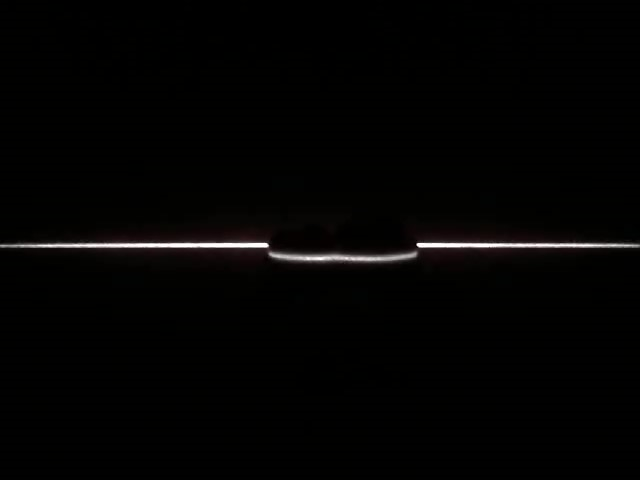
\includegraphics[width=0.4\textwidth]{frame_sample}
                \caption{Пример кадра из видео}
                \label{pic:frame_sample}
            \end{wrapfigure} 
            Перед тем как выделить на изображении лазер, необходимо провести предобработку, которая сгладит шумы в кадре и уберёт большинство лишней информации. Первым шагом необходимо обрезать видео по заранее установленной области интереса. Вне этой области заранее гарантировано отсутствие полезной информации, т.е. вне этой области нет рабочей зоны. 
            
            Затем к изображению применяется фильтр гаусса \cbox{пояснение что это?}, что размывает картинку. Это делается с целью <<размешать>> шум имеющийся на изображений и сгладить резкие переходы, что поможет на следующем шаге. 
            
            После этого с полученного изображения снимается <<маска>> -- то есть изображение бинаризируется. В таком изображении единицами обозначена область, которую мы хотим оставить, а нулями область, которую мы хотим отбросить. Для получения маски предусмотрено два подхода на выбор -- бинаризация по заданному пороговому значению и бинаризация с порогом по Оцу. Последняя хороша тем, что позволяет избежать необходимость ручного подбора порогового значения. 
            
            Метод Оцу применим к изображениям на гистограмме которых есть только два пика. Хорошее пороговое значение для таких изображений находится между этими двумя пиками\cite{opencvTHRESH}.
            
            Это идеально подходит для нашего случая. Такая маска единицами пометит области на изображении, в которых с наибольшей вероятностью находится лазер, а нулями области, где лазера почти наверняка нет.
            
            Последним шагом является применение маски к обрезанному изображению, что представляет собой простое поэлементное умножение. Таким образом мы получаем изображение, в котором область, где почти наверняка лазера нет, состоит из пикселей значение которых равно нулю, остальная же часть остаётся нетронутой.

            Это изображение затем передаётся в следующий блок алгоритма для выделения лазера.

        \subsection{Выделение лазера}
            Для постановки задачи выделения лазера в первую очередь необходимо определить, что из себя представляет линия лазера на изображении. В нашем случае линия лазера в кадре располагается параллельно оси $ X $ изображения. Интенсивность в профиле лазера, т.е. сечении в перпендикулярном ему направлении, соответствует Гауссовому\cite{Steger2000, Molder2014} с некоторым шумом. Пик интенсивности, без учета шума, соответствует центру полосы лазера.
            \begin{wrapfigure}{l}{0.4\linewidth}
                \centering
                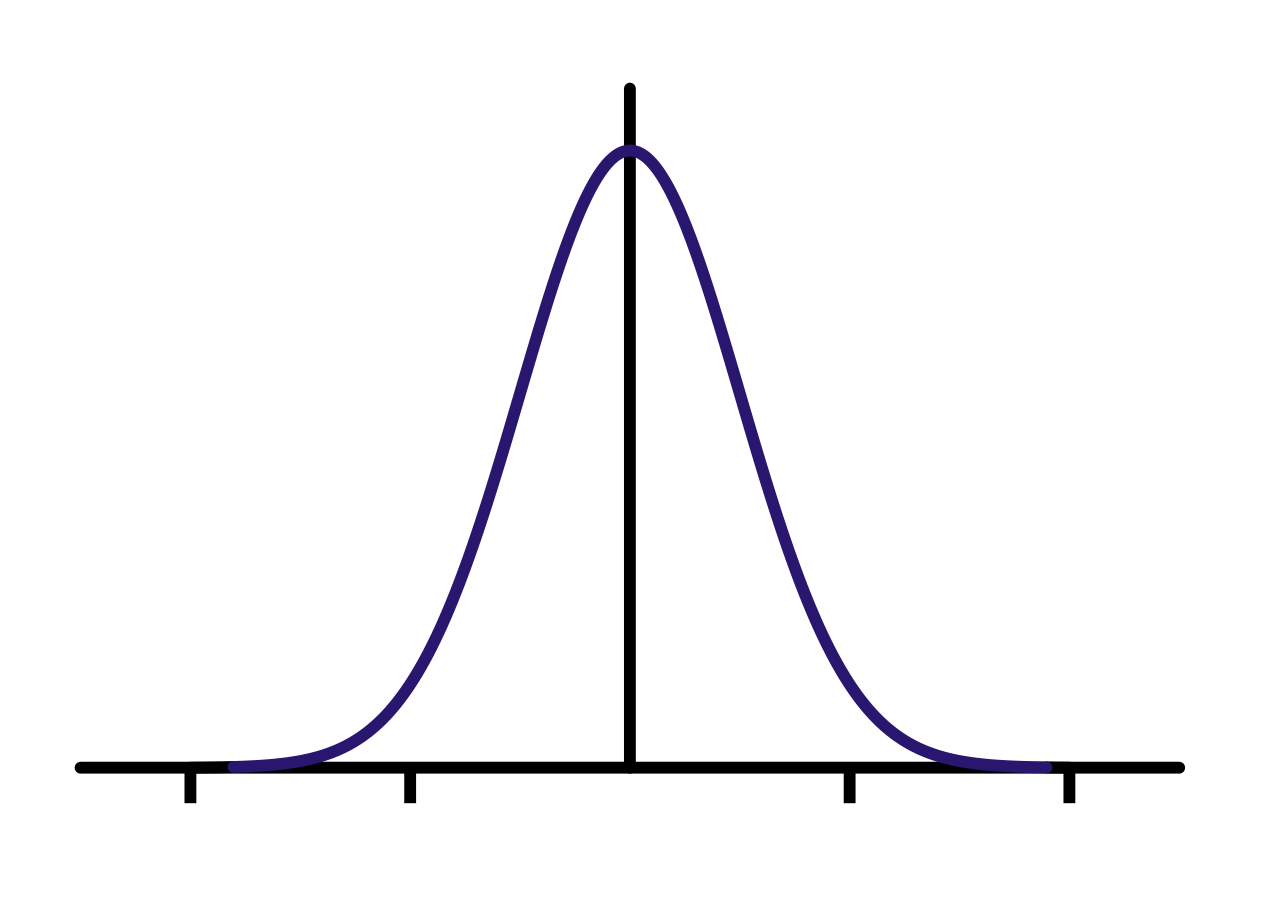
\includegraphics[width=0.38\textwidth]{gauss_profile}
                \caption{Распределение Гаусса}
                \label{pic:gauss_profile}
            \end{wrapfigure}
            Таким образом задача выделения лазера на изображении в итоге сводится к определению пика интенсивности для каждого профиля лазера, то есть в нашем случае для каждой колонки пикселей изображения.
            
            Однако задача усложняется наличием шумов на изображении, которые постоянно искажают профиль интенсивности лазера. Причинами шумов могут являться светочувствительный сенсор в камере, явление самозасвета лазера, неподходящие условия окружения, программная обработка изображения на этапе кодирования-декодирования и так далее.
            
            Помимо этого в общем случае линия лазера на изображении не является непрерывной. Разрывы могут возникать в следствии недостаточной контрастности лазера или попадания линии лазера в слепую зону. Эта проблема также требует какого-то решения.
            
            Рассмотрим существующие алгоритмы для выделения лазера на изображении и как они справляются с упомянутыми пробемами.
            
            \paragraph{Метод максимальной интенсивности}
            
            \paragraph{Laplacian of Gaussian}\cite{Molder2014}
            
            \paragraph{Квадратичная аппроксимация}\cite{Molder2014}
            
            \paragraph{Gray-Gravity Method}\cite{Li2017} \cbox{и как это по русски?}
            
            \paragraph{Improved Gray-Gravity Method}\cite{Li2017}
            
            \paragraph{Steger Analysis}\cite{Steger2000}
            
            \paragraph{Usamentiaga Method}\cite{Usamentiaga2012}
            
        \subsection{Привязка координат}
            Ранее было сказано, что в виду аппаратных ограничений видео сканирования в общем случае начинается в неопределённый момент перед рабочей зоной. При этом нет возможности узнать координату сканера в момент начала записи видео. Это порождает проблему несоответствия рассчитанных в процессе обработки координат и реальных. Таким образом необходимо разработать алгоритм, который позволял бы по данным с видео определить необходимое смещение координат.
            
            Основная идея такого алгоритма состоит в том, что необходима уникальная метка-идентификатор, имеющая заранее известную координату. Такая метка и алгоритм должны удовлетворять следующим требованиям:
            \begin{itemize}
                \item Лёгкое определение по входному видео
                \item Устойчивость к ложноположительным срабатываниям
                \item Лёгкое внедрение в конструкцию
                \item Минимальное влияние на общее время работы алгоритма
            \end{itemize}

            
            
    \section{Блок поиска объектов}
    
    \section{Блок обработки dxf}
    
    \section{Блок генерации gcode}